\subsection{最小上界与最大下界}

定义6. 设E是一个有序集，并设X是E的一个子集。E中的一个元素称为X在E中的最大下界或下确界（相应地，最小上界或上确界），如果它是X在E中的下界（相应地，上界）集合的最大（相应地，最小）元素。

给定有序集E的一个子集X，X在E中的最小上界（相应地，最大下界），当它存在时，记为

\[
\sup _ {\mathbf {E}} \mathbf {X} (\text { 分别   inf } _ {\mathbf {E}} \mathbf {X})
\]

或记为sup X（相应地，inf X），如果没有歧义的话。一个集合 \(\{x, y\}\) 的两个元素的最小上界（相应地，最大下界），当它存在时，记为sup \((x, y)\) （相应地，inf \((x, y)\) )。类似地，对于三个元素集合的上确界和下确界，等等。如果E的子集X有最大元素a，则a是X在E中的上确界。

如果X在E中有最大下界 \(a\) ，则 \(a\) 是关于E上相反序的X的最小上界。因此，在接下来的内容中，我们大多可以仅限于考虑最小上界的性质。

\minorheading{示例}

\begin{enumerate}
\def\labelenumi{(\arabic{enumi})}
\item
  在一个有序集合E中，空集 \(\phi\) 的上界集合显然就是E本身；因此 \(\phi\) 在E中有上确界当且仅当E有最小元素，此时该最小元素即为 \(\phi\) 的最小上界。
\item
  在集合 \(\mathfrak{P}(\mathbf{E})\) （集合 \(\mathbf{E}\) 的子集所成的集合，按包含关系排序）中，每个子集 \(\mathfrak{S}\) （ \(\mathfrak{P}(\mathbf{E})\) 的子集）都具有最小上界，即 \(\mathfrak{S}\) 中这些集合的并集，以及一个最大下界，即 \(\mathfrak{S}\) 中这些集合的交集。
\item
  设 E、F 为两个集合，并设 \(\Theta\) 是 \(\Phi(\mathbf{E}, \mathbf{F})\) 的子集，其中映射是从 E 的子集到 F 的映射族，按映射的延拓来排序（第 1 号，例 3）。对每个 \(u \in \Phi(\mathbf{E}, \mathbf{F})\) ，设 \(\mathbf{D}(u)\) 为 u 的定义域。一族属于 \(\Phi(\mathbf{E}, \mathbf{F})\) 的映射存在公共延拓的条件（第二章，§ 4，第 6 号，命题 7）表明 \(\Theta\) 在 \(\Phi(\mathbf{E}, \mathbf{F})\) 中有最小上界，当且仅当对于每一对元素 \((u, v)\) （ \(\Theta\) 的元素）我们有 \(u(x) = v(x)\) ，每当 \(x \in \mathbf{D}(u) \cap \mathbf{D}(v)\) 时。
\end{enumerate}

一个映射 \(f\) （从集合 \(A\) 到有序集 \(E\) 中的映射）称为具有最小上界，如果像 \(f(A)\) 在 \(E\) 中有最小上界；这个界随后称为 \(f\) 的最小上界，并记作 \(\sup_{x \in A} f(x)\) 。对于最大下界也有类似的定义。

特别地，如果 E 的子集 A 在 E 中具有最小上界，则该界是 A 到 E 的典范单射的最小上界，因此可以写成 sup x。

命题 4. 设 E 是一个有序集，A 是 E 的一个子集，且 A 在 E 中既有最大下界又有最小上界。若 A ≠ ∅，则 inf A ≤ sup A；若 A = ∅，则 sup A 是 E 的最小元素，inf A 是 E 的最大元素。

这直接由定义得出。

命题 5. 设 E 是一个有序集，A、B 是 E 的两个子集，且每个子集在 E 中都有最小上界（相应地，最大下界）。若 A ⊂ B，则 sup A ≤ sup B（相应地，inf A ≥ inf B）。

推论。设 \((x_{t})_{i\in I}\) 是某个有序集 \(E\) 的一个元素族，该族在 \(E\) 中有最小上界。如果 \(J\) 是 \(I\) 的一个子集，使得该族 \((x_{t})_{i\in J}\) 在 \(E\) 中有最小上界，我们就有 \(\sup_{i\in J}x_i\leqslant \sup_{i\in I}x_i\) .

命题6. 设 \((x_{i})_{i\in I}, (y_{i})_{i\in I}\) 是同一个指标集 I 索引的有序集 E 的两个元素族，并且满足 \(x_{i} \leqslant y_{i}\) （对于所有 \(i\in I\) ）。若两个族在 E 中都有最小上界，则 \(\sup_{i\in I} x_{i} \leqslant \sup_{i\in I} y_{i}\) .

因为 \(a = \sup_{i \in I} y_i\) 是由各 \(y_i\) 组成的集合的一个上界，所以 \(x_i \leqslant y_i \leqslant a\) 对所有 \(i \in I\) 都成立，从而 \(\sup_{i \in I} x_i \leqslant a\) .

命题7. 设 \((x_{t})_{t\in I}\) 是某个有序集 \(E\) 的元素族，并且设 \((J_{\lambda})_{\lambda \in I}\) 是指标集 \(I\) 的一个覆盖。假设每个子族 \((x_{t})_{t\in J_{\lambda}}\) 在 \(E\) 中有最小上界。对于该族 \((x_{t})_{t\in I}\) 在 \(E\) 中具有最小上界，其充分必要条件是该族 \(\left(\sup_{t\in J_{\lambda}}x_{t}\right)_{\lambda \in L}\) 在 \(E\) 中具有最小上界，此时我们有

\[
\sup _ {i \in I} x _ {i} = \sup _ {\lambda \in L} \left(\sup _ {i \in J _ {\lambda}} x _ {i}\right).\tag{1}
\]

令 \(b_{\lambda} = \sup_{i \in J_{\lambda}} x_i\) 。假设 \((x_i)_{i \in I}\) 具有最小上界 \(a\) 。则 \(a \geqslant b_{\lambda}\) （对于每一个 \(\lambda \in L\) ）（命题5的推论）。另一方面，如果 \(c \geqslant b_{\lambda}\) 对于每一个 \(\lambda \in L\) ，那么我们有 \(c \geqslant x_i\) 对于每一个 \(i \in I\) ，因为 \((J_{\lambda})_{\lambda \in L}\) 是 \(I\) 的一个覆盖；因此 \(c \geqslant a\) ，这证明了

\[
a = \sup _ {\lambda \in L} b _ {\lambda}.
\]

反之，假设该族 \((b_{\lambda})_{\lambda \in \mathbf{L}}\) 具有最小上界 \(a'\) 。则 \(a' \geqslant x_{i}\) 对于所有 \(i \in I\) 。另一方面，如果 \(c' \geqslant x_{i}\) 对于所有 \(i \in I\) ，那么我们特别有

\[
c ^ {\prime} \geqslant \sup _ {i \in J _ {\lambda}} x _ {i} = b _ {\lambda}
\]

对于每一个 \(\lambda \in \mathbf{L}\) ，因此 \(c' \geqslant a'\) ，从而

\[
a ^ {\prime} = \sup _ {i \in I} x _ {i}.
\]

推论。设 \((x_{\lambda \mu})_{(\lambda, \mu) \in \mathbf{L} \times \mathbf{M}}\) 是某个有序集合 \(\mathbf{E}\) 的一个“双重”元素族，使得对于每一个 \(\mu \in \mathbf{M}\) ，族 \((x_{\lambda \mu})_{\lambda \in \mathbf{L}}\) 在 \(\mathbf{E}\) 中有最小上界。该族 \((x_{\lambda \mu})_{(\lambda, \mu) \in \mathbf{L} \times \mathbf{M}}\) 在 \(\mathbf{E}\) 中具有最小上界的充分必要条件是，族 \(\left(\sup_{\lambda \in \mathbf{L}} x_{\lambda \mu}\right)_{\mu \in \mathbf{M}}\) 在 E 中具有最小

上界，此时我们有

\[
\sup _ {(\lambda , \mu) \in L \times M} x _ {\lambda \mu} = \sup _ {\mu \in M} \left(\sup _ {\lambda \in L} x _ {\lambda \mu}\right).\tag{2}
\]

命题8. 设 \((\mathbf{E}_t)_{t \in I}\) 是一族有序集。设 A 是乘积有序集 \(\mathbf{E} = \prod_{t \in I} \mathbf{E}_t\) 的一个子集，并且设 \(\mathbf{A}_t = \operatorname{pr}_t \mathbf{A}\) （对于每一个 \(t \in I\) ）。要使 A 在 \(\mathbf{E}\) 中有最小上界，必要且充分的条件是：对每个 \(t \in I\) , \(\mathbf{A}_t\) 在 \(\mathbf{E}_t\) 中有最小上界，此时我们有

\[
\sup A = (\sup A _ {t}) _ {t \in I} = \left(\sup _ {x \in A} \operatorname{pr} _ {t} x\right) _ {t \in I}.
\]

假设对于每一个 \(t \in I\) , \(A_t\) 具有最小上界 \(b_t\) （在 \(E_t\) 中）. 要说 \(c = (c_t)\) 是 \(A\) 的一个上界，那就意味着 \(c_t \geqslant b_t\) 对于每一个 \(t \in I\) 成立，因此 \((b_t)_{t \in I}\) 是 \(A\) 的一个上界。相反，假设 \(A\) 具有最小上界 \(a = (a_t)_{t \in I}\) ；对于每个 \(x \in I\) , \(a_x\) 是 \(A_x\) 的一个上界，因为如果 \(x_x \in A_x\) , 就存在 \(x \in A\) 使得 \(pr_x x = x_x\) ，这由 \(A_x\) 的定义可得；另一方面，如果 \(a_x'\) 是 \(A_x\) 在 \(E_x\) 中的一个上界，那么元素 \(c' = (c_t')_{t \in I}\) （对于它）

\[
c _ {i} ^ {\prime} = a _ {i} \quad \text { 对 } \quad i \neq x \quad \text { 且 } \quad c _ {x} ^ {\prime} = a _ {x} ^ {\prime}
\]

是A的一个上界；于是 \(c' \geqslant a\) ，因而 \(a_{x}' \geqslant a_{z}\) ；因此 \(a_{x}\) 是 \(A_{x}\) 在 \(E_{x}\) 中的最小上界.

\pandocbounded{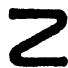
\includegraphics[keepaspectratio]{images/part002_f683a60c9eaa907b29b9c0e21fae4a1da7b4dd647e1d1a410962ae330fdaf4f4.jpg}}

设F是有序集E的一个子集，并设A是F的一个子集。可能发生两个元素 \(\sup_{E} A\) , \(\sup_{F} A\)

示例

中的一个存在而另一个不存在，或者两者都存在但不相等。* (1) 在实数有序集 \(\mathbf{E} = \mathbf{R}\) （实数集）中，考虑有理数子集 \(\mathbf{F} = \mathbf{Q}\) 以及有理数集 \(\mathbf{A} \subset \mathbf{F}\) ，即满足 \(< \sqrt{2}\) 的有理数所成的集； \(\sup_{\mathbf{E}} \mathbf{A}\) 存在但 \(\sup_{\mathbf{F}} \mathbf{A}\) 不存在。

\begin{enumerate}
\def\labelenumi{(\arabic{enumi})}
\setcounter{enumi}{1}
\item
  在例1的记号中，设G为A与集合 \(\{2\}\) 的并集；那么 \(G \subset F\) ，并且 \(\sup_{G} A\) 存在，但 \(\sup_{F} A\) 不存在。
\item
  使用相同的记号， \(\sup_{\mathbf{E}} \mathbf{A} = \sqrt{2}\) , \(\sup_{\mathbf{G}} \mathbf{A} = 2\) . *
\end{enumerate}

然而，我们有以下结果：

命题9. 设E是一个有序集，F是E的一个子集，A是F的一个子集。如果 \(\sup_{\mathbf{E}}\mathbf{A}\) 与 \(\sup_{\mathbf{F}}\mathbf{A}\) 都存在，我们有 \(\sup_{\mathbf{E}}\mathbf{A} \leqslant \sup_{\mathbf{F}}\mathbf{A}\) 。如果 \(\sup_{\mathbf{E}}\mathbf{A}\) 存在且属于F，则 \(\sup_{\mathbf{F}}\mathbf{A}\) 存在且等于 \(\sup_{\mathbf{E}}\mathbf{A}\) .

第一个断言由以下事实得出：A在F中的上界集合M包含于A在E中的上界集合N，以及命题5。另一方面，如果N的最小元属于F，则它属于M，并且显然是M的最小元；这证明了第二个断言。

